\documentclass[11pt]{report}

\special{papersize=8.5in,11in}

\topmargin -0.5in \oddsidemargin 0.00in \evensidemargin 0.00in
\textwidth 6.75in \textheight 9.0in \headheight 0.25in \headsep
0.25in \footskip 0.5in \hoffset 0in \marginparpush 0.0in
\marginparwidth 0.0in \marginparsep 0.2in

\setcounter{page}{1}

\newcommand{\D}{\displaystyle}\newcommand{\T}{\textstyle}
\newcommand{\e}{{\mathrm{exp}}}
\newcommand{\dd}{{\mathrm d}}
\newcommand{\comment}[1]{}
\newcommand{\mb}{\mathbf}
\reversemarginpar
\usepackage{bm}
\usepackage[final]{graphicx}
\usepackage{fancyhdr}
%\graphicspath{{Papers/}}
\usepackage{amsthm,amssymb,amsmath}
\usepackage{cite}
\usepackage{geometry}
\usepackage{amsmath}
\usepackage{booktabs}
\usepackage{color}
\usepackage{setspace}
\usepackage{subfigure}
\usepackage{url}
%\usepackage{algorithm}
\usepackage{algorithmic}
\usepackage[ruled]{algorithm2e}
\usepackage{multirow}
\usepackage{tabularx}

%\usepackage[top=2.5cm, bottom=2.5cm, right=3.5cm, left=3.5cm]{geometry}
\geometry{a4paper,scale=0.8}
\setcounter{secnumdepth}{3}

\title{Research Progress Report}

\author{Botao Zhu}

\begin{document}
	
	\maketitle
	\lhead{\sf Research Progress Report-10th} \chead{} \rhead{\sf Botao Zhu}
	\lfoot{CTRG, University of Saskatchewan} \cfoot{} \rfoot{Page \thepage}
	\renewcommand{\footrulewidth}{1.0pt}
	\renewcommand{\headrulewidth}{2.0pt}
	\renewcommand{\arraystretch}{1.3}
	\pagestyle{fancy}
	
	\renewcommand{\thesection}{\arabic{section}}
	
	\section{Reading and Research Activities}
 
	


	\textbf{An improved soft K-means clustering protocol for balancing energy in wireless sensor networks}\\
	
	%%%%
	% there are a few research on Leach for non-uniform area. the most of modified leach protocol focus on savig energy and extedning the lifetime of wsn. mainly on following aspects: 1. improving the selection of ch, like considering residual energy  2.improving clustering methods, like kmeans. in detail, comparing kmeans with other algorithms, the initial centroid, . 3.choosing two or more chs in the cluster. 4. controlling normal nodes to send data.
    \noindent \textbf{Abstract} \\
    Energy load balance is the essential issue in designing the wireless sensor networks (WSNs). Clustering technique is utilized as an energy-efficient routing to balance the network energy and prolong the lifetime, which is influenced by the cluster head selection and clustering method. In this paper, we propose an approach based on the idea clustering by fast search and ind of density peaks (CFSFDP) and kernel density estimation (KDE) to optimize the selection of the initial cluster heads of clustering algorithm. And then, we use reassigning member nodes and multi-heads scheme to balance the energy consumption of all nodes in the whole network. Simulation results demonstrate that the proposed approach can postpone the first node death by almost 3 times and the half of nodes death by 2 times compared to LEACH. Also, smoother energy distribution curve of all nodes in different round and smaller energy variance are obtained by our proposed algorithm.
	
	\subsection{Introduction}
	
	Energy limitation is a key challenge in WSNs, since nodes' batteries cannot be rechargeable or nodes are placed in areas where it hard to reach to replace batteries. So, energy consumption is an important design issue for WSNs \cite{7539358}. Clustering in energy limited WSNs has been widely pursued in order to solve energy issue of sensor networks. The clustering-based algorithm groups sensor nodes into distinct clusters with a head in a cluster and each sensor node belongs to only one cluster. All member nodes sense environment information and send it to the cluster heads (CHs), the CHs collect and process the data and send it to the base station (BS) via single-hop or multi-hop \cite{7855660}. Each node consumes a certain amount of energy when it collects, processes, and sends data. A node is defined to be dead when it is out ot energy\cite{8632891}. Hence, it is crucial to find efficient clustering algorithms to balance the energy consumption among sensor nodes in WSNs.\\
	
	\noindent Machine Learning-based clustering algorithms are considered to be the most effective clustering methods in WSNs. Reference \cite{6375088} implements both centralized and distributed K-means clustering algorithm in WSNs. EEK-means\cite{quchan2016towards} creates symmetric clusters and reduces the average intra-cluster communication distance by the K-means classification method in order to save energy of nodes and improve the network lifetime.  K-LEACH protocol \cite{Sangameswaran}  prolongs the lifetime of sensor networks by balancing the nodes' energy consumption, which uses K-medoids for clustered WSNs. Reference  \cite{rabiaa2015improvements} uses K-means and Gauss algorithms to achieve the optimization of energy consumption of a network and the extension of its duration of life. 
	\\
	%\noindent Most of the research literature on WSNs are based on the assumption that the sensor nodes are randomly distributed throughout the entire network \cite{7588902,8252252}, which will result in a non-uniform distribution of the sensor nodes. The main problem of clustering of non-uniformly distributed sensors is that it can increase the energy consumption of WSNs. In \cite{5693275,doi:10.1155/2013/289527}, the authors propose W-LEACH algorithm to handle non-uniformly distributed nodes in the network. In order to extend the WSNs lifetime, it only chooses a number of sensors in each cluster to send data to their CHs based on a fixed percentage, which can reduce the traffic load of CHs. However, it may result in the loss of important information. Hence, it is crucial to study clustering for non-uniformly distributed nodes in WSNs.\\
	
	%\noindent K-means clustering algorithm is very useful to produce clusters, which tries to find a specified number of clusters and minimize the sum of Euclidean distances between the head and member nodes\cite{macqueen1967}. It is used in LEACH to achieve better classification performance compared to the traditional LEACH\cite{6375088}. However, the K-means algorithm suffers from the following drawbacks. First, the K-means algorithm chooses the initial centroid randomly, which cannot ensure the clustering result is optimal. If the initial centroids are far away from the true centroid of clusters, it will increase the number of iterations until convergence. Second, the node with the highest residual energy in the cluster is elected as the CH and this can lead to a potential problem: unbalanced energy load and excessive energy expenditure. For example, if the node CH1 in Fig. \ref {cha} has higher residual energy than other nodes in cluster A, then CH1 has high probability to be elected as the CH. However, this way enables the other nodes in the same cluster to send data in the opposite direction to the BS, causing higher energy consumption. 
	%\begin{figure}[!h]
	%	\centering
	%	\includegraphics[width=0.3\linewidth]{cha.eps}
	%	\caption{A example of clustering}
	%	\label{cha}
	%\end{figure}
	 %Third, the K-means does not consider that some of sensor nodes in a cluster can be reallocated to other clusters for balancing the size of different clusters. As shown in Fig. \ref{cha}, node $N$ belongs to cluster A by applying hard classification, K-means. Since the density of cluster A is greater than that of cluster B, node $N$ can be re-allocated to cluster B in order to reduce the stress of CH of cluster A. 
	 %Fourth, in K-means, each cluster selects only one cluster head, so the energy of cluster head will be depleted quickly for aggregating, compressing, and transmitting information when there are too many sensor nodes in the cluster. %\cite{Sangameswaran} proposed a method to prolong the lifetime of each round by balancing the energy consumption of among nodes in the network. The nodes are divided into three types in each cluster: CH, vice CH and member nodes. The vice CH plays the role of CH when the CH dies before the completion of current round, which can diminish the frequency of re-clustering and extend network lifetime. \cite{doi:10.1155/2016/5040475} also comes up with a similar concept. Three nodes in each cluster are selected as CHs to ensure the load is evenly balanced in different clusters. However, if these two methods are applied to non-uniform distributed wireless networks, the problem of energy balance is still unsolved. \\
	
	
    
    \noindent In this paper, an improved soft K-means (ISK-means) clustering protocol is proposed. Specifically, the main contributions of this paper are as follows.\\ 
    1) Compared with some existing cluster-based protocols that select CH randomly, we choose the initial centroids of soft K-means clustering algorithm \cite{report} by using the idea of density from clustering by fast search and find of density peaks (CFSFDP), which is implemented by kernel density estimation (KDE). \\
    2) According to the characteristics of soft K-means, reallocating member nodes that locate in the boundary of two or more clusters is employed to balance the number of nodes in different clusters. \\
    3) Since the clustering process needs to be repeated continually, it can increase the communication cost during the period of clustering. Multi-heads method is used to balance traffic load of CHs of different clusters and reduce the frequency of clustering.\\
    
    \noindent The rest of this paper is organized as follows: Section \uppercase\expandafter{\romannumeral2} reviews the related works. The background for our research are described in Section \uppercase\expandafter{\romannumeral3}. Section \uppercase\expandafter{\romannumeral4} proposes the implementation of the proposed ISK-means algorithm. In section \uppercase\expandafter{\romannumeral5}, we compare the performance of the proposed ISK-means with other routing algorithms. Finally, the paper is concluded in Section \uppercase\expandafter{\romannumeral6}.
    
    \subsection{Related works}
    
    Different clustering techniques have been proposed in designing WSNs to obtain energy efficiency and maximize network lifetime. Low energy adaptive clustering hierarchy (LEACH) is one of the first energy efficient routing protocols, proposed by Heinzelman et al. \cite{926982}. In this protocol, it selects CHs using a threshold among nodes by rotation and other nodes choose the nearest CH to form cluster, which can spread energy dissipation to all nodes in the network. However, it may result in a nonuniform distribution of CH thus causing high energy consumption. Low energy adaptive clustering hierarchy centralized (LEACH-C) \cite{1045297} is the modified version of LEACH. In LEACH-C, each node sends its current location and residual energy to BS. BS determines the number of CH and arranges network into various clusters, which can ensure that load is eventually distributed in different clusters. However, this centralized approach can increase communication overhead during the period of selection of CH. Energy-aware clustering algorithm \cite{6602412} considers two factors: the energy factor for cluster head selection and distance factor for non-cluster heads to select its cluster head, which achieves a good performance in terms of lifetime by balancing the energy load among all the sensor nodes in the network. 
	\\
	
     \noindent K-means clustering algorithm is used in WSNs, which tries minimize the sum of Euclidean distances between the head and member nodes according to a specified number of clusters \cite{6375088}. Due to selection of CHs randomly, it can result in sub-optimal clusters and uneven distribution of load. Reference \cite{randhawa2016performance} proposes a modified K-means algorithm that considers two factors: distance between CHs and its member nodes and remaining energy of nodes to reduce energy consumption and extend the lifespan compared to LEACH. BPK-means \cite{4622679} balances the clusters to improve intra-cluster communication consumption, which can achieve better load-balance. In \cite{mahboub2017energy}, the authors propose a hybrid clustered routing algorithm based on K-means clustering algorithm and LEACH protocol, which outperforms LEACH in terms of energy consumption. However, it can increase energy consumption during the phase of CH election process. EECPK-means \cite{7763028} balances the load of CHs in WSNs by producing balanced clusters where midpoint method is used to improve the initial centroids selection of K-means algorithm.
     
     %is used to group the nodes and CHs are chosen depending on their distance from cluster center and residual energy. But, with the random deployment of the nodes, K-means may result in vagueness of classifying nodes near the boundary of the clusters. \\ 
     
     %In order to minimize the sum of Euclidean distances between the head and member nodes, 
     
     %\cite{6550511} provides a novel way to choose cluster heads by using K-means method for maximizing the energy efficiency of WSN. However, this algorithm may cause different kinds of clusters in different runs based on the chosen initial centroids randomly. 
	%Energy-aware clustering approach based on K-means (KEAC) \cite{gachhadar2014k} provides less energy consumption throughout the whole network. It chooses cluster heads according to remaining energy and distance from their centroids and achieves low energy consumption. However, the adjustment of the ratio to communicate with BS may increase the overhead. \\
	
	
	%\noindent Most of the deployment in WSN is random, where sensor nodes are distributed unevenly and the number of nodes is not uniform in each cluster. Some efforts are made to come up with some solutions regarding the uniform distribution of load and to achieve energy efficiency through non-uniform deployment of nodes.
	%\cite{1420160} proposed an unequal clustering size (UCS) model for network organization, which can lead to more uniform energy dissipation among the cluster head nodes, thus increasing network lifetime. Area covered by the clusters can be altered in each layer by changing radius of a layer near to BS and hence will change density of a particular cluster. The drawback of this approach is the number of nodes in each cluster may vary to a great extent.
	 %A new model for non-uniform deterministic node distribution is proposed \cite{6785530} that reduces the total number of nodes to be deployed over the area and the network traffic satisfying both coverage and load balancing criteria. The simple distributed algorithm is introduced to load balanced data gathering. However, this approach may cause energy hole problem. \cite{7489086} proposed fuzzy based unequal clustering protocol (FUCP), which is a novel clustering algorithm which incorporate CH selection algorithm by using fuzzy logic and relay traffic distributed to eliminate hot spot problem. It has more longer network lifetime and sends more packets to BS compared to distributed energy efficient hierarchical clustering. Energy degree distance unequal clustering algorithm (EDDUCA)\cite{Guiloufi2016} aims to balance energy consumption and maximize the network life, which use 'Sierpinski' method to divide the network into unequal clusters. The results indicate that EDDUCA can effectively balance the energy consumption. Energy-aware clustering algorithm (EAC) \cite{6602412} considers two factors: the energy factor for cluster head selection and distance factor for non-cluster heads to select its cluster head, which achieves a good performance in terms of lifetime by balancing the energy load among all the sensor nodes in the network. An energy-aware clustering and cluster-based routing algorithm \cite{YU201254} uses competition range to construct clusters of even size for nonuniform deployment of sensor nodes to balance the load across the entire network. The cluster head is selected on the basis of the ratio of average remaining energy of nearby nodes and the energy of node itself, which achieves load balance among cluster heads.
	 
	 \subsection{PRELIMINARIES}
	 
	\subsubsection{Soft K-means}
	\cite{report} K-means is the simplest clustering algorithm in unsupervised learning, which partitions the data set in to $k$ clusters using some distance measurement methods, like Euclidean distance. It is a hard clustering method, that is to say the membership degree of one node has only two values 0 and 1 for a specific class. However, in some cases, there are a few data points for which it is not quite so obvious to which cluster they belong. Soft K-means clustering decides to which degree each data point belongs to , the assignments to clusters will be probabilistic. Generally speaking, soft K-means clustering can be seen as the problem of finding $k$ cluster centroids with the aim of minimizing the error function. Given a set of data points $X = \{x_1,x_2,...,x_n\}$, the error function is
	
	\begin{equation}
	E\left(\mu_1,\mu_2,...,\mu_k\right) = \sum_{i=1}^{k}E\left(\mu_i\right) = \sum_{i=1}^{k}\sum_{j=1}^{n}z_{ij} ||x_j-\mu_i||^2
	\end{equation}
	where $\mu_i$ is the centroid of each cluster, $z_{ij}$ is the indicator variable. \\ 
	For the traditional K-means clustering 
	\begin{equation}
	z_{ij} = \left\{ \begin{array}{ll}
	1, \text{if}\,x_{j} \in C_{i}\\
	0, \text{otherwise}
	\end{array} \right.
	\end{equation}
	where $C_{i}$ represents cluster $i$, this equation means whether $x_{i}$ belongs to cluster $C_{i}$. However, $z_{ij}$ is not a integer value for soft K-means clustering 
	\begin{equation}
	\label{eq1}
	z_{ij} = \frac{e^{-\beta ||x_{j}-\mu_i||^2}}{\sum_{l=1}^{k}e^{-\beta||x_{j}-\mu_l||^2}}
	\end{equation}
	where $\beta$ is the stiffness parameter, its impact for clustering result will be discussed in simulation section. 
	From equation (\ref{eq1}), we can get $z_{ij} \in [0,1]$ and $\sum_{i}z_{ij}=1$.\\
	How to update the centroid $\mu_{i}$ of each cluster until convergence? For a specific class $C_{i}$
	\begin{equation}
	\label{eq2}
	E\left(\mu_{i}\right) = \sum_{j=1}^{n}z_{ij}||x_{j}-\mu_{i}||^2
	\end{equation}
	The target is to minimize the error function, so the problem can be turned into the following optimization problem
	\begin{equation}
	e = \text{argmin}\sum_{j=1}^{n}z_{ij}||x_{j}-\mu_{i}||^2
	\end{equation}
	which is a convex function and has a unique minimum value. The equation (\ref{eq2}) can be written as
	\begin{eqnarray}
	E\left(\mu_{i}\right) &=& \sum_{j=1}^{n}z_{ij}\left(x_j-\mu_{i}\right)\top \left(x_j-\mu_{i}\right)\\
	 &=& \sum_{j=1}^{n}z_{ij}\left(x_j \top x_j-2x_j \top \mu_{i} + \mu_{i} \top \mu_{i}\right)
	\end{eqnarray}
	deriving $E\left(\mu_{i}\right)$ with respect to $\mu_{i}$ and denoting to zero, we can have
	\begin{equation}
	\label{eq3}
	\mu_{i} = \frac{\sum_{j=1}^{n}z_{ij}x_j}{\sum_{j=1}^{n}z_{ij}}
	\end{equation}
	Each cluster updates the centroid according to equation (\ref{eq1}) and (\ref{eq3}) until the probabilities of the clusters in which the data points are located remain unchanged or the maximum number of iterations are reached. \\

	%\noindent The advantage of applying soft K-Means clustering in wireless sensor network is each sensor node joins the clusters with a certain probability, which can prevent some clusters from having too many nodes. Assuming two adjacent cluster A and B, the number of nodes in cluster A is greater than that in cluster B, shown in Fig.\ref{fig1}. It will lead to a serious case that the cluster head node of cluster A consumes energy quickly because cluster head node will take more energy to deal with the message from member nodes within its cluster. In this case, some nodes at the intersection edge of cluster A and B will join cluster B with greater probability to reduce the stress of cluster head node of cluster A in order to avoid energy hole. However, the random selection of initial clustering centroid makes the clustering results fall into local optimum, and the accuracy of soft K-Means algorithm is low because of the noise points and the uncertain clustering. 
	
	\subsubsection{Kernel density estimation}
	The first law of geography states that all things are interrelated. The closer they are, the stronger they are. Kernel density estimation is based on this law, its value decreases gradually with the increase of the central radiation distance. From two-dimensional or three-dimensional surface of density, we can intuitively acquire the features of point sets \cite{1990}. 
	
	For an observation value $x$ of random variable $X$, the probability that it falls into the interval $[a, b]$ can be computed by
	\begin{equation}
	\label{eq9}
	P = \int_{a}^{b}\hat{p}\left(x\right)dx
	\end{equation}
	where $\hat{p}$ is the probability density function. When $|b-a|\ll \varepsilon$, $\varepsilon \to 0$, equation (\ref{eq9}) becomes to 
	\begin{equation}
	P = \hat{p}\left(x\right)\int_{a}^{b}dx = \hat{p}\left(x\right)\left(b-a\right)
	\end{equation}
	Hence
	\begin{equation}
	\hat{p} = \frac{P}{b-a}
	\end{equation}
	If there are k observation value of n falling into the interval $[a, b]$, the probability will be 
	\begin{equation}
	P = \frac{k}{n}
	\end{equation}
	the probability density function
	\begin{equation}
	\hat{p} = \frac{k}{n\left(b-a\right)}
	\end{equation}
	We define the kernel function
	\begin{equation}
	\label{14}
	K\left(u\right)  = \left\{ \begin{array}{ll}
	1, |u|\leq\frac{1}{2}\\
	0, \text{otherwise}
	\end{array} \right.
	\end{equation}
	Assuming the center of interval $[a,b]$ is $x$ and $h=b-a$, any sample $x_i$ falling into the interval $[a, b]$ needs to meet the following requirement.
	\begin{eqnarray}
	|x-x_i| &\leq& \frac{b-a}{2}\\
	\label{16}
	\frac{|x-x_i|}{h} &\leq& \frac{1}{2}
	\end{eqnarray}
	From equation (\ref{14}) and (\ref{16}), we can obtain
	\begin{equation}
	K\left(\frac{x-x_i}{h}\right) = \left\{ \begin{array}{ll}
	1, |\frac{x-x_i}{h}| \leq \frac{1}{2}\\
	0, \text{otherwise}
	\end{array} \right.
	\end{equation}
	So, the value k can be expressed by 
	\begin{equation}
	k = \sum_{i=1}^{n}K\left(\frac{x-x_i}{h}\right)
	\end{equation}
	and then, 
	\begin{equation}
	\label{19}
	\hat{p}\left(x\right)=\frac{1}{nh}\sum_{i=1}^{n}K\left(\frac{x-x_i}{h}\right)
	\end{equation}
	which is the kernel density function. 
	
	
	\noindent \cite{reportkernel} \cite{doi:10.1080/02331880500439782}Kernel density is one of the non-parametric estimation methods used to estimate the unknown density function. Each point is covered with a smooth surface. The surface value at the location of the point is the highest and decreases with the increase of distance until the value is zero when the distance equals the search radius, which looks like the density map of Gauss distribution function. Then, the values of kernel density estimation of all points are superimposed and a set of points is transformed into a surface showing continuous density changes. Fig.\ref{fig22} is an example of kernel density estimation for a non-uniform distribution network. The discrete point set is transformed into a smooth density map, shown in Fig.\ref{3d}, which shows its spatial distribution. The higher the density value, the higher the aggregation degree of the point is.\\
	\begin{figure}[!h]
		\subfigure[original data distribution]{
			\begin{minipage}[h]{0.5\linewidth}
				\centering
				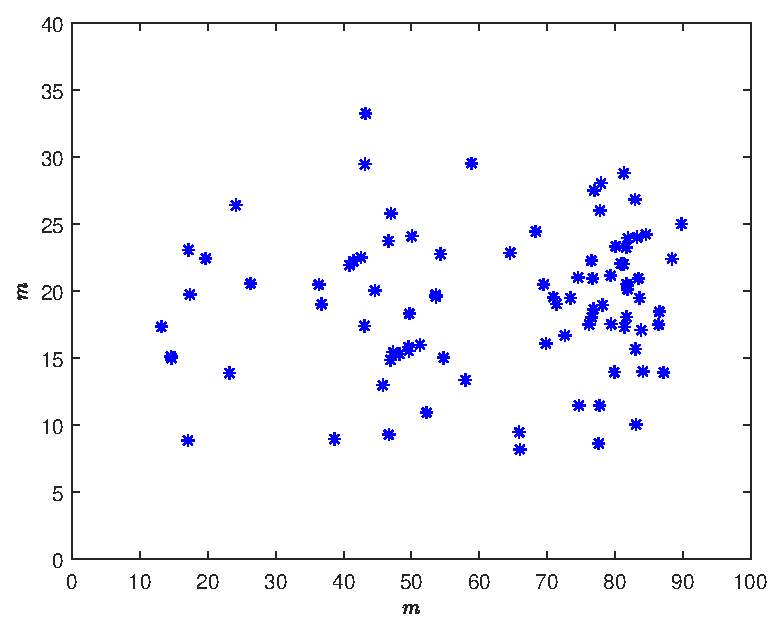
\includegraphics[width=3in]{original.eps}
				\label{original}
			\end{minipage}
		}%
	    \subfigure[Denstiy contour of original data]{
	    	\begin{minipage}[h]{0.5\linewidth}
	    		\centering
	    		\includegraphics[width=3in]{density.eps}
	    		\label{3d}
	    	\end{minipage}
	    }
		\centering
		\caption{A example of kernel density estimation}
		\label{fig22}
	\end{figure}
	%\noindent Firstly, the data samples are estimated by their position attributes to obtain a image which can show continuous density changes. The pixel value of the image represents the density of the location in the data samples. Setting a threshold, the image is divided into high-density areas and low-density areas. Then, the highest density points are extracted in some high density ares to form maximum density point set. Maximum density point set is used as clustering center, and the number of maximum density point set is used as K value. The maximum density points in a certain region are obtained, but the clustering effect is not good with the points in the low density region, so the maximum density point set is only obtained in the high density region.

    \subsection{Proposed Algorithm}
	\subsubsection{Network Model}
	We have following assumptions regarding the network model \cite{article} \cite{7763028}:\\
	(a) The BS is a high energy node and is located far away from the extremities of the sensor network.\\
	(b) All sensor nodes having the same computational and transmission capabilities. In other words, all nodes are capable of acting as CH nodes.\\
	(c) The sensor nodes can vary the power with which they transmit signals according to the received signal strength indication of a particular node.\\
	(d) The sensor nodes scans its environment at a fixed rate and will contain data to be sent to the BS at all intervals.\\
	(e) The sensor nodes and BS are all static after deployment.\\
	(f) The sensor nodes in general have location information such as a GPS support.\\
	(g) The CHs perform data compression to reduce the amount of bits transmitted to the BS.\\
	(h) The BS indicates all nodes to reinitiate clustering when all the CH nodes in the network have insufficient energy.
	
	\subsubsection{Energy model}
	
	Because the main energy consumption of the protocol is only for receiving and sending data, the first order radio model as the energy model is in line with the needs. The consumption energy in the transmitter nodes and in the receiver node can be calculated as follows:
	\begin{equation}
	E_{T}=\left\{ \begin{array}{ll}
	l * E_{elec} + l * \varepsilon_{fs} * d^2 & d \leq d_0 \\
	l * E_{elec} + l * \varepsilon_{mp} * d^4 & d > d_0 \\
	\end{array} \right.
	\end{equation}
	\begin{equation}
	E_R = l * E_{elec}
	\end{equation}
	where $E_{elec}$ is the dissipated energy per bit in both transmitter nodes and receiver nodes, $d$ is the transmission distance and $d_0$ is defined as the distance threshold, $d_0 = \sqrt{\frac{\varepsilon_{fs}}{\varepsilon_{mp}}}$, $l$ is the packet size. The free space $\varepsilon_{fs}$ and multipath fading channel $\varepsilon_{mp}$ represent the energy consumption parameters of amplifier, which one can be used depends on the distance between the transmitter and the receiver. 
	
	If the transmission distance $d_{toBS}$ between the cluster head and the sink node is larger than $d_0$ and the distance between member node and the cluster head $d_{toCH}$ is less then $d_0$, the energy consumption of cluster head can be calculated in this round by
	\begin{equation}
	\label{22}
	E_{CH} = k*l*c*\left(E_{T} + E_{DA} + \varepsilon_{mp}*d^4_{toBS}\right) + k*l*E_R
	\end{equation}
	where $E_{DA}$ represents the dissipated energy of data aggregation and $c$ is the data aggregation ratio. The first part of equation (\ref{22}) is the energy consumption of the cluster head for sending aggregated data to the sink node and the second part is the energy consumption of receiving and aggregating data of k member nodes. The energy consumption of a non-cluster node sending data to the cluster head by
	\begin{equation}
	E_{nonCH} = l * E_T + l * \varepsilon_{fs} * d^2_{toCH}
	\end{equation}
	Hence, the residual energy of node $i$ in each round $r$ can be computed by
	\begin{equation}
	\label{24}
	E_i\left(r\right)=\left\{ \begin{array}{ll}
	E_i\left(r-1\right) - [ k*l*c*\left(E_{T} + E_{DA} + \varepsilon_{mp} * d^4_{toBS}\right) + k*l*E_R]& i \in CH \\
	E_i\left(r-1\right) - l * E_T + l * \varepsilon_{fs} * d^2_{toCH} & i \notin CH \\
	\end{array} \right.
	\end{equation}
	where $E_i\left(r-1\right)$ is the residual energy for node $i$ in the $r-1$ round and $CH$ is the cluster heads.\\


	 Routing protocols can be classified many types, such as flat protocol and hierarchy protocol. The proposed protocol belongs to hierarchy protocol, which is divided into many rounds, like LEACH. Each round contains setup phase and steady phase. In this research, we only focus on the setup phase and improve some existing methods. During the setup phase,  the sink node gathers the location and residual energy of each node in the whole wireless network. Also, it generates k initial centers by CFSFDP and KDE as the input of ISK-means clustering algorithm, which can avoid the local optimum by traditional K-means clustering method. And then, classification algorithm is implemented. Each node calculates the distance between itself and center points and chooses to join the nearest cluster with a certain probability. At the same time, if the nodes on the edge of two clusters have similar distance to these two cluster centers, they will preferentially join the cluster with smaller density. After clustering, the final CHs are selected according to the energy. The detailed discussion is given below.
	
	\subsubsection{Selection of Initial Cluster Heads}
	 
	 \cite{Rodriguez1492} discovered that clusters can be recognized regardless of their shape and the dimensionality of the space in which they are embedded. The basic idea is that cluster centers are surrounded by neighbors with lower local density and they are at a relatively large distance from any points with a higher local density. Hence, the larger the number of nodes in its neighborhood is, the higher the value of local density will be. The cluster heads are selected by the maximum distance $\sigma$ and relatively high local density $p$.\\
	 
	 \noindent In this paper, we use the similar idea of density maximum to select the initial cluster heads. However, we only consider the density parameter $p$, which can be obtained by KDE. The nodes with highest local density will be chosen as the cluster heads, because the area with the larger number of nodes can easily form the maximum local density in non-uniform distribution wireless networks.
	 \begin{equation}
	 	\text{N}_{p_{max}} = \text{max}\left(\text{N}_{\hat{p}_i}\right), i \in \text{local region nodes}
	 \end{equation}
	  According to above equation, we can obtain a maximum density node set $\{\text{N}_{p_{max1}},\dots,\text{N}_{p_{maxK}}\}$. After the number of maximum density regions, $K$, is determined, each normal node joins the nearest cluster head with higher density to form initial clusters by CFSFDP algorithm. Then, the nodes with the largest energy in each initial cluster are selected as the input of improved soft K-means clustering algorithm. There are several benefits through the above steps to ensure the initial cluster heads: (1) the number of clusters k is determined by maximum density principle. (2) the distances between the greatest energy nodes of each cluster are relatively large. The detailed description is shown in algorithm 1. 
	 
	 \begin{algorithm}[H]
	 	\caption{Selection of initial cluster heads}
	 	\label{alg1} 
	 	\LinesNumbered %show number
	 	\KwIn{the set of $n$ data items $\mb{X} = \{x_1,x_2,\dots,x_n\}$}
	 	\KwOut{initial cluser heads set}
	 	\For{i = $\mathrm{1,2}$,\dots,n}{calculate $p_i$ by equation (\ref{19})}
	 	obtain density set $P = \{p_1,\dots,p_n\}$ \\
	 	get local maximum density node set $\{\text{N}_{p_{max1}},\dots,\text{N}_{p_{maxK}}\}$ by statistical tool as the initial cluster heads\\
	 	each member node joins its cluster head $\text{N}_{p_{maxK}}$ via CFSFDP algorithm to form $K$ initial clusters $\{C_1,\dots, C_K\}$\\
	 	\For{j = $\mathrm{1:}$ K}{calculate the highest energy nodes of $C_j$}
	 	the set of the highest energy nodes of each cluster $\bm{\mu} = \{\mu_1,\dots,\mu_K\}$
	 \end{algorithm}
	
	
	\subsubsection{Cluster Formation}
	 
	 Machine learning has been widely used in wireless sensor networks for forming cluster, such as distributed K-means clustering algorithm \cite{7425183}, improved K-means cluster-based routing\cite{8379004} and LEACH-CKM \cite{6987570}. The above algorithms are based on the distances between normal nodes and cluster head nodes to form clusters, which can easily lead to a large gap in the number of different clusters in non-uniform distribution networks. Furthermore, the energy consumption of cluster head nodes is not balanced. Hence, compared with these K-means clustering algorithms, our proposed algorithm uses soft K-means clustering algorithm. Each node is assigned a probability of belonging to cluster head rather than completely being a member of just one cluster. Therefore, the nodes close to the boundary of clusters may have the similar probabilities belonging to different clusters. And, we also take one more step after the classification convergence, assigning nodes at the edge of different clusters to join the approximate cluster for balancing the number of normal nodes in clusters. We discuss this problem in two scenarios.\\
	 
	 \noindent \textbf{Scenario 1:} The node N is at the edge of two clusters, shown in Fig. \ref{fig5}. The distance from node N to the center of cluster B is a little bigger than that from node N to the center of cluster A, which means it has a higher probability to join cluster A. However, it is a different story if we consider the densities of different clusters. Cluster A has 5 member nodes and cluster B has 10 member nodes. Assuming that all normal nodes send messages to its CH in each round, CH of cluster B will deal with more information from its member nodes. In order to balance the energy consumption of CHs, it is better for node N to join cluster A. Here, we give a simple definition of re-assigning nodes. When the difference of probability of a node belonging to two clusters is less than 25$\%$, the node will join the cluster with low density.\\
	 \noindent \textbf{Scenario 2:} The node N is at the boundary of three or more clusters, shown in Fig.\ref{fig6}. After clustering, each node will have a probability set representing the possibilities of belonging to different clusters, $\bm{z}_i = \{z_{i1},z_{i2}, \dots z_{iK} \}$. The cluster of the node belonging to with low probability will not be considered. So, we only choose the first two maximum probabilities and calculate their difference, $D_i$. If $ D_{i} < 10\%$, the node will join the cluster with smaller density between two maximum probability clusters. As shown in Fig. \ref{fig6}, node N has similar probability belonging to cluster A, B and C, which finally joins cluster C because cluster C has lower density than cluster A and B.  
	 
	 \begin{algorithm}[H]
	 	\caption{Cluster formation}
	 	\LinesNumbered %show number
	 	\KwIn{
	 		\\Initial cluster heads $\bm{ \mu} = 
	 		\{\mu_1,\dots,\mu_K\}$ from \textbf{algorithm} \ref{alg1}\\
	        Data items $ \mathbf{X} = \{x_1,x_2,\dots,x_n\}$\\
            Iterations $r_{max}$}
	 	\KwOut{ \\$K$ clusters}
	 	\For{$r$ = $\mathnormal{1} : r_{max}$}
	 	{\For{i = $\mathnormal{1}:n$}
	 		{$z_{ik} = \frac{e^{-\beta||x_i-\mu_k||^2}}{\sum_{K}e^{-\beta||x_i-\mu_k||^2}}$}
	 		$\mb{z}={
	 			\left[ \begin{array}{cccc}
	 				z_{11} & z_{12} & \cdots & z_{1K}\\
	 				\vdots & \vdots & \vdots & \vdots\\
	 				z_{i1} & \cdots & \cdots & z_{iK}
	 			\end{array} 
	 			\right ]}$\\
 		    \For{k = $\mathnormal{1}:K$}
 		    {$\mu_k = \frac{\sum_{i=1}^{n}z_{ki}x_{i}}{\sum_{i=1}^{n}z_{ki}}$}
 	    }
     	K clusters $\bm{C} = \{C_1,\dots,C_K\}$ \\
     	\For{i = $\mathnormal{1}:n$}
     	{check $z_i$ and reassign the node $i$ by scenario 1 and 2}
     	K clusters $\bm{C}_{new} = \{C_{new1},\dots,C_{newK}\}$ \\	
	 \end{algorithm}
 \begin{figure}[h!] 
 	\centering
 	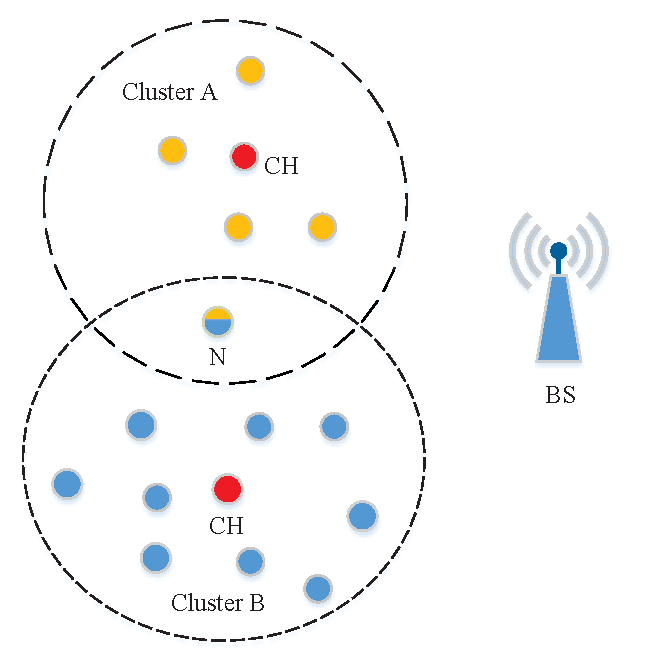
\includegraphics[width=0.35\linewidth]{cha3.eps}
 	\caption{Node at the boundary of two clusters}
 	\label{fig5}
 \end{figure}
 \begin{figure}[h!]
 	\centering
 	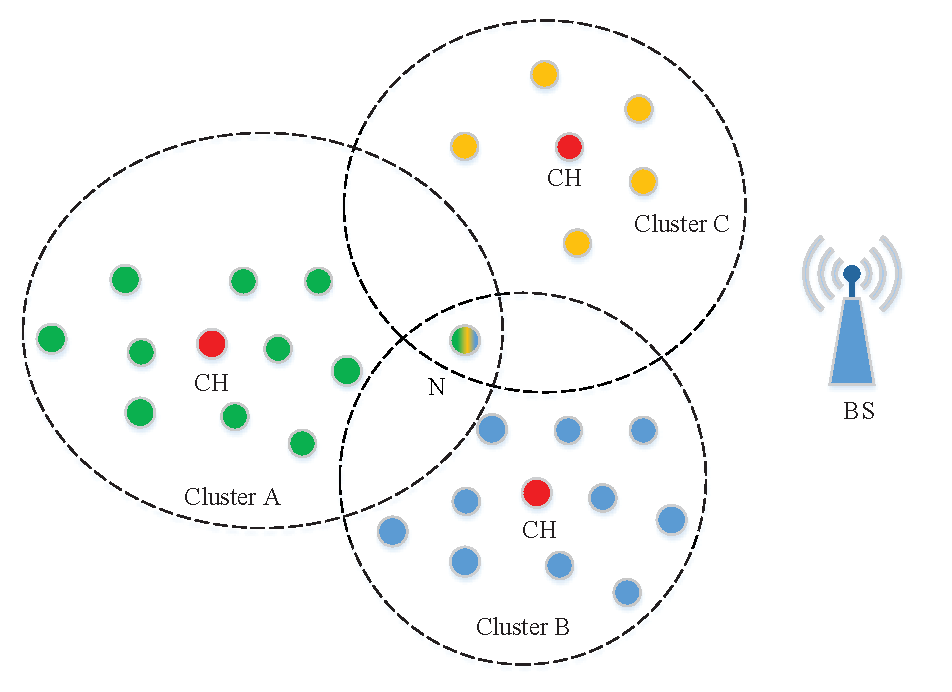
\includegraphics[width=0.5\linewidth]{cha2.eps}
 	\caption{Node at the boundary of three clusters}
 	\label{fig6}
 \end{figure}
	\subsubsection{Selection of Final Cluster Heads}
	%The most common way to select cluster heads is to choose the nodes with the largest residual energy, which may cause excessive energy consumption. In this step, we still use kernel density estimation to select cluster heads and add a parameter $\sigma$ in $\hat{f}(x)$, which represents the residual energy of node. Equation (\ref{eq19}) can ensure that CHs are selected in the area with the highest energy density.\\
	%\begin{equation}
	%\label{eq19}
	%\hat{f}(x) = \frac{\sigma}{nh} \sum_{i=1}^{n}K\left(\frac{x-x_i}{h}\right)
	%\end{equation}
	
	%At the same time, the number of cluster head nodes is not fixed in each cluster, which is determined by the nodes in the cluster. Here we give a simple rule. We count the nodes of each cluster and sort in descending order of size. The first 30\% clusters takes three head nodes, the middle 30\% clusters takes two head nodes and the last 30\% clusters takes one head node. This method can avoid the communication overhead caused by frequent clustering and take into account the different size of clusters.
	In non-uniform distributed wireless sensor networks, the cluster size will be different. If only one CH is selected for each cluster, CH will consume too much energy to deal with the information from its member nodes in the large cluster, which will cause its death too early. Hence, our proposed algorithm designs the scheme of multi-cluster heads. The number of cluster head nodes is not fixed in each cluster, which is determined by the number of the nodes in the cluster. The larger of the number of nodes in the cluster is, the more the number of CH will be. In a cluster, the nodes which have more remaining energy and close to the center are preferentially selected as CHs. The total remaining energy of cluster $k$ can be computed by:
	\begin{equation}
	E\left(k\right)_{total} = \sum_{i=1}^{S_k}E_i\left(r\right)
	\end{equation}
	where $S_k$ is the size of cluster $k$, $E_i\left(r\right)$ is the residual energy of node $i$ in current round, which can be obtained by equation (\ref{24}).\\
	The average energy of cluster $k$ is:
	\begin{equation}
	E_{ave} = \frac{E\left(k\right)_{total}}{S_k}
	\end{equation}
	\noindent This scheme can balance the energy consumption of cluster heads of different cluster in non-uniform distributed wireless sensor networks, shown in Fig.\ref{fig7}. \\
	
	\begin{algorithm}[h!]
		\caption{Selection of final cluster heads}
		\LinesNumbered %show number
		\KwIn
		{\\K clusters $\mb{C}_{new} = \{\text{C}_{new1},\dots,\text{C}_{newK}\}$ }
		\KwOut{\\$K$ cluster heads}
		\For{k = $\mathnormal{1}:K$}
		{Calculating the size of cluster $\text{C}_{newk}$, $S_k$\\
		Calculating average energy of cluster $E_{ave}$\\
		$Num = \frac{S_k}{constant}$, the number of CHs of cluster\\
		\For{i = $\mathnormal{1}:S_k$ }
		{Iterating $x_i$ from near the center of cluster\\
			
			\If{$E_i > E_{ave}$ and $Num > 0$}
			{$Num = Num - 1$\\
		    $\text{CH}_k\left(Num\right) = x_i$}}
        }
		K cluster heads $\mb{CH} = \{\text{CH}_1,\dots,\text{CH}_K \}$
	\end{algorithm}
	\begin{figure}[h!]
		\centering
		\includegraphics[width=0.25\linewidth]{multihead.eps}
		\caption{Multi-heads scheme}
		\label{fig7}
	\end{figure}
	\subsubsection{Switching Cluster Head}
	
	\noindent In the first round, the first node in $\text{CH}_k$ is selected as the current CH for cluster $k$. After CHs for the current round are selected, the sink node notifies all nodes to join the cluster to which they belong. CHs broadcast TDMA schedules to their member nodes for transmitting data in different time slots to avoid data collision. Then, the network is in a steady phase and begins to exchange data between normal nodes and their CHs. For balancing the energy consumption of CH, when the energy of current CH of any cluster is below the threshold value, the next candidate CH in that cluster is enabled. Until all CH in the cluster are executed, the algorithm starts re-clustering.\\
	
	\begin{algorithm}[H]
		\caption{Switching cluster head mechanism}
		\LinesNumbered %show number
		\KwIn
		{\\K cluster heads $\mb{CH} = \{\text{CH}_1,\dots,\text{CH}_K \}$}
		\KwOut{\\
		Next cluster head}
		Current round\\
		\For{k = $\mathnormal{1}:K$}
		{$\rho = \frac{\text{the residual energy of}\,  \text{CH}_k \,\text{last round}}{\text{the residual energy of}\,  \text{CH}_k \,\text{current round}}$\\
		\If{$\rho < \text{Threshold}$}
		{
		    \eIf{$\text{CH}_k$ has next}{switching next CH}{reclustering}}}
	\end{algorithm}
	
    \subsection{Experiment results and analysis}
    \subsubsection{Simulation settings}
	The simulation is executed in MATLAB R2017a. Sensor nodes are deployed in an area of $100 \times 100 m^2$, the sink node is located at $(50m,150m)$. The main parameters are shown in Table \ref{table1}. 

	\begin{table}[h!]
		\centering
		\caption{Simulation parameters}
		
		\label{table1}  
		\begin{tabular}{p{4cm}p{3cm}}
			\toprule[1.5pt]
			\textbf{Parameter} & \textbf{Value}\\
			\hline
			Area & $100m \times 100m$  \\
			\hline
			Sink node & (50,150)\\
			\hline
			Initial energy & 0.2J,1J\\
			\hline
			Packet length & 4000bits\\
			\hline
			Control length & 100bits\\
			\hline
			$E_T$ & 50nJ/bit \\
			\hline
			$E_R$ & 50nJ/bit \\
			\hline
			$\varepsilon_{fs}$ & 10pJ/bit\\
			\hline
			$\varepsilon_{mp}$ & 0.0013pJ/bit\\
			\hline
			$E_{DA}$ & 5nJ/bit\\
			\hline
			$d_0$ & 88m\\
			\hline
			Number of sensor nodes & 26,100\\
			\bottomrule[1.5pt]
		\end{tabular}
	\end{table}
    \subsubsection{Reassigning nodes of improved soft K-means analysis}
    In this section, we will discuss the impact of reassigning nodes scheme of improved soft K-means for balancing energy consumption of CH. A non-uniform distributed network with 26 nodes is generated. Firstly, we use K-means classification method to classify these nodes and get two clusters, shown in Fig.\ref{K-Means classification result}. It is found that cluster 1 contains 19 nodes, which is much higher than cluster 2. As a result, CH of the heavily loaded cluster, which contains 26 nodes will be exhausted much earlier than another cluster. Fig.\ref{Soft K-Means classification result} shows the similar classification result by soft K-means method when $\beta$ is 0.3, which can not balance the number of different clusters very well. However, we find that the nodes on the edge of two clusters have similar probabilities belonging to these two clusters, like node 1, node 2, node 3, node 4 and node 5. At the same time, when the value of $\beta$ changes, the probabilities also change. Table \ref{table2} lists the probabilities of the above nodes belonging to different clusters and their change for different $\beta$. In section 1.2, we know $\beta$ represents stiffness parameter, which is the tightness of node belong to a cluster. As can be seen from Table \ref{table2}, 
    when $\beta = 1$, all five nodes belong to the cluster with a higher probability than the case, $\beta = 0.3$. Hence, the larger the value of $\beta$, the closer the nodes is associated with a cluster. We set $\beta= 0.3$ in the simulation for using the ISK-means algorithm better. According to the principles described in scenario 1, node 2, node 3, node 4 and node 5 are reassigned to cluster 2 from cluster 1, which balances the number of these two clusters. The residual energy of CH, computed by equation (\ref{24}), in each round could be used to check the result and advantage of this scheme. Fig.\ref{Resiadual energy of CHs after 5 rounds} and Fig.\ref{Resiadual energy of CHs after 10 rounds} show that both K-means and soft K-means result in unbalanced energy consumption of CH, however, the ISK-means method achieves an equilibrium of energy consumption in both CH.
    
	\begin{figure}[!h]
	\subfigure[K-means classification result]{
		\begin{minipage}[h]{0.5\linewidth}
			\centering
			\includegraphics[width=3in]{fig11.eps}
			\label{K-Means classification result}
		\end{minipage}
	}%
	\subfigure[Soft K-means classification result]{
		\begin{minipage}[h]{0.5\linewidth}
			\centering
			\includegraphics[width=3in]{fig8.eps}
			\label{Soft K-Means classification result}
		\end{minipage}
	}
	\subfigure[ISK-means classification result]{
		\begin{minipage}[h]{0.5\linewidth}
			\centering
			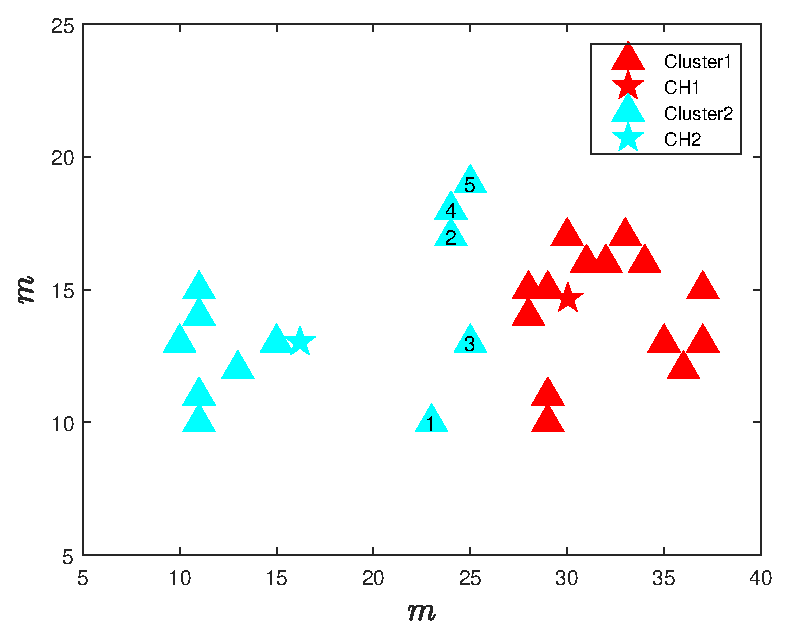
\includegraphics[width=3in]{fig9.eps}
			\label{Improved soft K-Means classification result}
		\end{minipage}
	}%
	\centering
	\caption{Comparison of different classification methods}
	\label{}
	\end{figure}

	\begin{table}[h!]
		\centering
		\caption{Probabilities comparison}
		\label{table2}  
		\begin{tabular}{c|c|c|c|c|c|c}
			\toprule[1.0pt]
			\multicolumn{2}{c|}{Probability} & Node 1 & Node 2 & Node 3 & Node 4 & Node 5\\
			\hline
			\multirow{2}*{$\beta = 0.3$} & Cluster 1 & 0.4852 & 0.5537 & 0.5684 & 0.6120 & 0.6120 \\
			\cline{2-7}
			& Cluster 2 & 0.5148 & 0.4463 & 0.4316 & 0.3880 & 0.3880
			\\
			\hline
			\multirow{2}*{$\beta = 1$} & Cluster 1 & 0.0438 & 0.9787 & 0.9860 & 0.9992 & 0.9992 \\
			\cline{2-7}
			& Cluster 2 & 0.9562 & 0.0213 & 0.014 & 0.0008 & 0.0008\\
			\bottomrule[1.5pt]
		\end{tabular}
	\end{table}

	\begin{figure}[!h]
		\subfigure[Resiadual energy of CHs after 5 rounds]{
			\begin{minipage}[h]{0.5\linewidth}
				\centering
				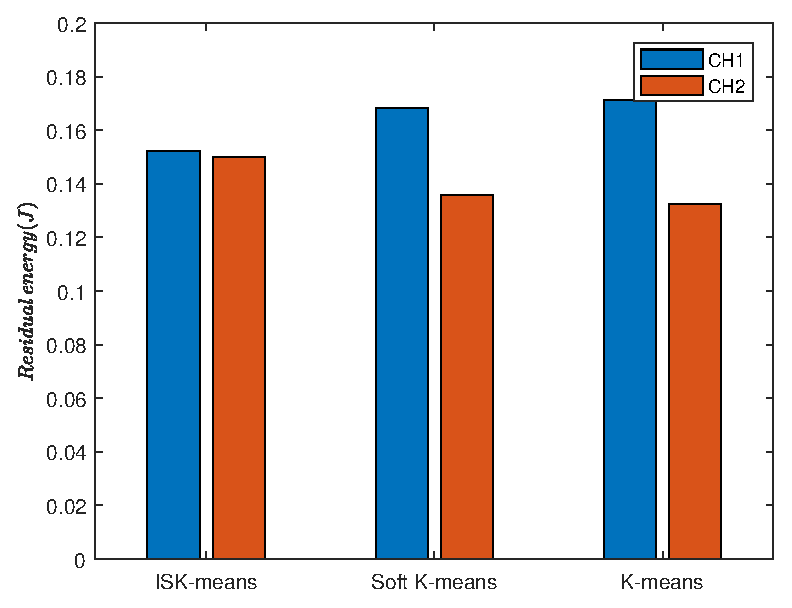
\includegraphics[width=3in]{energy10.eps}
				\label{Resiadual energy of CHs after 5 rounds}
			\end{minipage}
		}%
		\subfigure[Resiadual energy of CHs after 10 rounds]{
			\begin{minipage}[h]{0.5\linewidth}
				\centering
				\includegraphics[width=3in]{energy15.eps}
				\label{Resiadual energy of CHs after 10 rounds}
			\end{minipage}
		}
		\centering
		\caption{Comparison of residual energy of CHs}
		\label{}
	\end{figure}
	
	\subsubsection{Network lifetime}
    To test the performance of ISK-means, we compare it with LEACH \cite{1045297} and K-means \cite{6375088}. Fig.\ref{fig9} shows the first node death(FND), half of nodes death(HND) and the last node death(LND) for three methods when the number of nodes is 100 and the area is $100m \times 100m$. If the protocol can balance energy very well, the first node death will be very late. In this paper, we assume that the death of 95\% nodes means all nodes dead. In view of Fig.\ref{fig9} and Fig.\ref{fig10}, the sensor nodes lifetime of our proposed algorithm is better than that of LEACH and K-means. For K-means, the round of FND is 191, which is much earlier than 962 in LEACH and 2663 in ISK-means. However, the LND in K-means happens later compared with LEACH. It is obvious that the energy consumption of K-means is unbalanced, this is because K-means algorithm selects the initial cluster heads randomly, which is sensitive to noise and abnormal data, especially in non-uniform distributed wireless networks. The proposed ISK-means algorithms takes energy into account. The result shows it can effectively postpone the FND, HND and LND. The FND of ISK-means is 2663, which is about 3 times that 962 of Leach and 14 times of K-means. The HND is also around 2 times of both LEACH and K-means, which means ISK-means can balance the energy consumption of the network effectively. Obviously, ISK-means can keep most of the nodes alive in the network, so that the existence of the death of first nodes happens later. As a result, 

	\begin{figure}[h!]
		\centering
		\includegraphics[width=0.7\linewidth]{three.eps}
		\caption{Comparison of network lifetime}
		\label{fig9}
	\end{figure}

	\begin{figure}[h!]
		\centering
		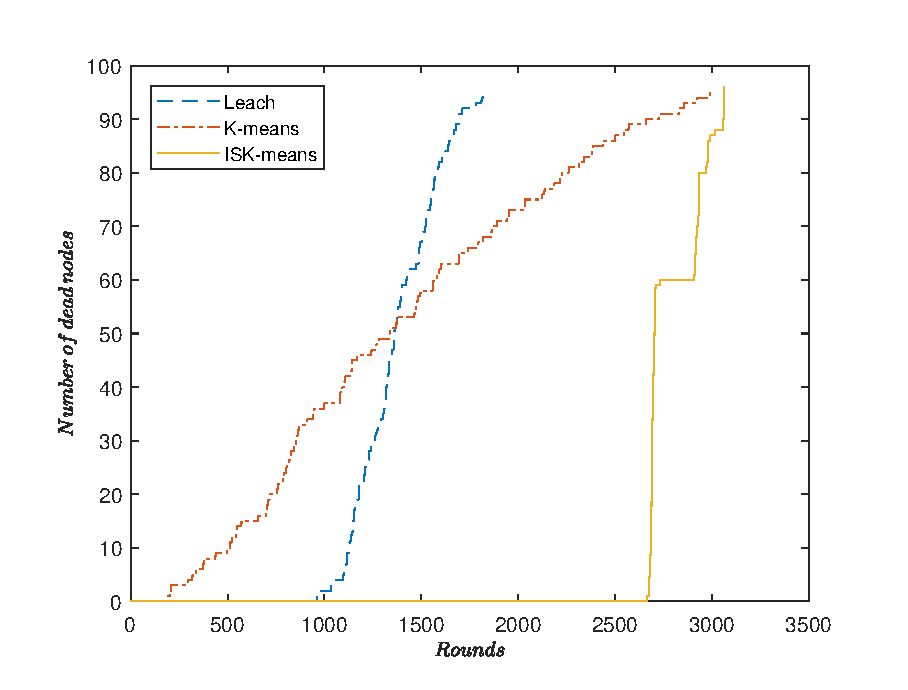
\includegraphics[width=0.7\linewidth]{nodedead.eps}
		\caption{Comparison of node death curve}
		\label{fig10}
	\end{figure}

	\subsubsection{Received packets at BS}
	Fig.\ref{fig11} shows the received packets at BS for among three algorithms. Because of using multi-heads scheme in ISK-means, the number of re-clustering decreases, which reduces the communication cost of clustering between CHs and their member nodes. As a result, data transmission frequency increases and more packets are successfully transmitted to the BS compared to that in LEACH and K-means.
	
	\begin{figure}[h!]
		\centering
		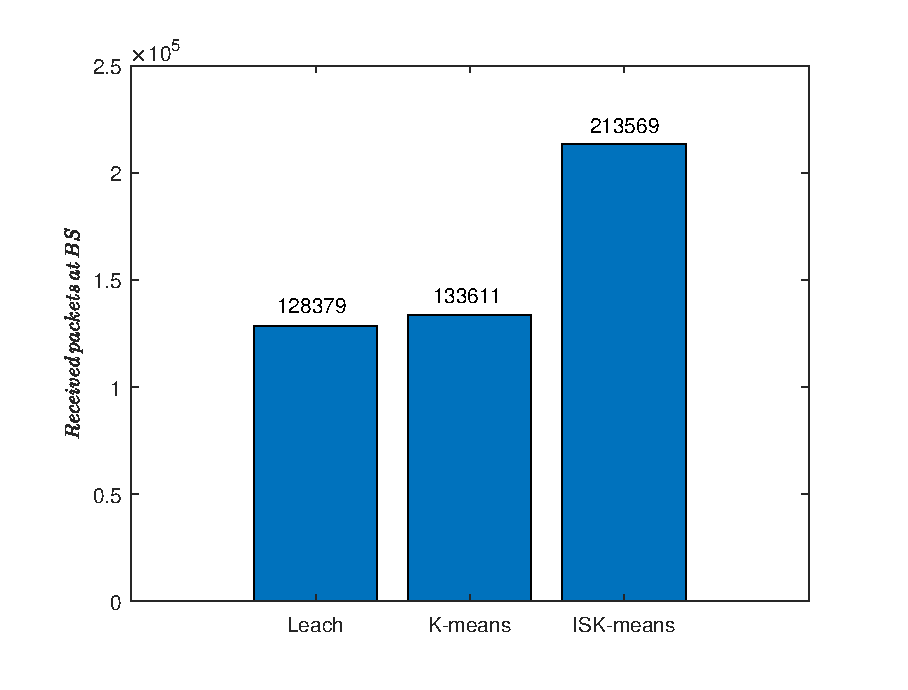
\includegraphics[width=0.7\linewidth]{packet1.eps}
		\caption{Received packets at BS}
		\label{fig11}
	\end{figure}
	\subsubsection{Energy Variance}
	
	Fig.\ref{fig12} shows the comparison of residual energy of all 100 nodes in the network for among three algorithms after different rounds.  It is found that the energy distribution curve of all nodes by using ISK-means protocol is smoother than that of LEACH and K-means, and the curve of K-means is the worst. This result demonstrates that ISK-means is good at balancing energy consumption of all nodes in the whole network. \\
	For purpose of estimating the performance of proposed algorithm, we denote a new parameter: energy variance(EV), can be expressed by
	\begin{equation}
	\sigma^2 = \frac{\sum_{i=1}^{n}\left(E\left(x_i\right) - \overline{E}\right)^2}{n}
	\end{equation}
	where $E\left(x_i\right)$ is the energy of node $i$ in current round and $\overline{E}$ is the average energy of all nodes. In table \ref{table3}, it clearly reveals that ISK-means obtains smaller variances than LEACH and K-means in different rounds, which demonstrates that ISK-means can keep the energy distribution of 100 nodes in the network to be the most uniform.
	
	\begin{figure}[!h]
		\subfigure[Residual energy after 200 rounds]{
			\begin{minipage}[h]{0.5\linewidth}
				\centering
				\includegraphics[width=3.3in]{node500.eps}
				\label{Residual energy after 200 rounds}
			\end{minipage}
		}%
		\subfigure[Residual energy after 600 rounds]{
			\begin{minipage}[h]{0.5\linewidth}
				\centering
				\includegraphics[width=3.3in]{node700.eps}
				\label{Residual energy after 600 rounds}
			\end{minipage}
		}
		\subfigure[Residual energy after 1000 rounds]{
			\begin{minipage}[h]{0.5\linewidth}
				\centering
				\includegraphics[width=3.3in]{node900.eps}
				\label{Residual energy after 1000 rounds}
			\end{minipage}
		}%
		\subfigure[Residual energy after 1400 rounds]{
			\begin{minipage}[h]{0.5\linewidth}
				\centering
				\includegraphics[width=3.3in]{node2000.eps}
				\label{Residual energy after 1400 rounds}
			\end{minipage}
		}
		\centering
		\caption{Comparison of residual energy distribution}
		\label{fig12}
	\end{figure}
	
	\begin{table}[h!]
		\centering
		\caption{Comparison of energy variance in different rounds}
		\label{table3}  
		\begin{tabular}{c|c|c|c|c|c|c|c|c}
			\toprule[1pt]
			\multirow{2}*{} & \multicolumn{8}{c}{Variance}\\
			\cline{2-9}
			& 200 r & 400 r & 600 r & 800 r & 1000 r & 1200 r & 1400 r & 1600 r\\
			\hline
			LEACH & 0.0011 & 0.003 & 0.0062 & 0.0108 & 0.017 & 0.017 & 0.0088 & 0.0026\\
			\hline
			K-means & 0.0345 & 0.0752 & 0.1043 & 0.1194 & 0.1158 & 0.1028 & 0.0907 & 0.0659
			\\
			\hline
			ISK-means & 0.00028 & 0.0005 & 0.0007 & 0.00083 & 0.001 & 0.0011 & 0.0013 & 0.0016\\
			\bottomrule[1pt]
		\end{tabular}
	\end{table}


	\subsection{Conclusions}
	In this paper, we propose an energy balanced ISK-means algorithm protocol based on soft K-means for non-uniform distributed wireless sensor networks.  Firstly, it optimizes the selection of initial cluster heads of soft K-means clustering method by CFSFDP and KDE algorithms and a better cluster formation is obtained. Secondly, in order to balance the size of different clusters in non-uniform networks,  we use the soft classification characteristics of soft K-means to reassign some nodes locating at the boundary of different clusters to smaller size cluster.  Furthermore, multi-heads scheme is used in the selection of final cluster heads, which can effectively balance the traffic load of cluster heads, reduce the number of re-clustering and save communication cost. Experiments have demonstrated that ISK-means algorithm can balance energy very well for all nodes in the network during the period of network survival and the amount of data transmitted to the BS is increased remarkably. 
	
	
	
	
	
	
	
	
	
	~~~~~~~~~~~~~~~~~~~~~~~~~~~~~~~~~~~~~~~~~~~~~~
	
	\section{Objectives for the Next 2 Weeks}
	Simulate the algorithm proposed above.
										
	
	
	\section{Advisor's Comments}
	
	\bibliographystyle{IEEEtran}
	\bibliography{janbib}
	
\end{document}